\documentclass[a4paper, 11pt, fleqn, leqno]{article}

\usepackage[brazil]{babel}
\usepackage[utf8]{inputenc}

\usepackage[
paperheight=10.5in,
paperwidth=8.27in,
bindingoffset=0in,
left=0.8in,
right=1in,
top=1in,
bottom=1in,
headsep=1.5\baselineskip,
%showframe,% just for the example
]{geometry}

\usepackage{float}
\usepackage{comment}
\usepackage{hyperref}

\usepackage[colorinlistoftodos]{todonotes}
\usepackage{graphicx,varwidth}
\usepackage{xcolor}

%\usepackage{indentfirst}
\usepackage{gensymb}
\usepackage{amsmath,amssymb,amsthm,amsfonts,amsxtra}
\usepackage{verbatim}
\usepackage{textcomp}

\usepackage[printwatermark]{xwatermark}

\usepackage{listings}

%\newwatermark*[allpages,color=blue!10,angle=45,scale=1.5,xpos=0,ypos=0]{RAFAEL DOMINGUES}

\begin{document}
	
	\begin{center}
		\begin{tabular}{@{}c@{}}
			\includegraphics[width=2.5cm]{imagens/logo}
		\end{tabular}%
		\hfill
		\begin{varwidth}{\textwidth}
			\centering\bfseries
			{\large Universidade Federal de Itajubá - UNIFEI/MG \\
				Mestrado Acadêmico em Física}
		\end{varwidth}%
		\hfill
		\begin{tabular}{@{}c@{}}
			\includegraphics[width=2.5cm]{imagens/logo}
		\end{tabular}%
	\end{center}

\begin{center}
	
	\vspace{3cm}

	\textbf{\Huge \textbf{Fotometria de Galáxias: \\ \vspace{1cm} Perfil de Brilho de De Vaucouleurs}}
	
	\vspace{3cm}
	
	\textbf{\huge \textbf{Rafael Passos Domingues}}
	
	\vspace{1cm}
	
	{\Large d2021101072@unifei.edu.br}
	
	\vspace{5cm}
	
	\large{\today}	
	
\end{center}

\newpage
\tableofcontents
\newpage

%\begin{figure}[H]
%	\centering
%	\includegraphics[scale=0.6]{imagens/nomedafigura}
%\end{figure}

\newpage

\section{Resumo}

Foi ajustado o perfil de brilho das galáxias $NGC ~ 3522$ e $NGC ~ 5628$ do catálogo de De Vaucouleurs, de 1991. Os dados das galáxias escolhidas foram obtidos no \textit{VizieR}\footnote{VizieR fornece a biblioteca mais completa de catálogos astronômicos publicados --tabelas e dados associados - com dados verificados e enriquecidos, acessíveis através de múltiplas interfaces. As ferramentas de consulta permitem ao usuário selecionar tabelas de dados relevantes e extrair e formatar registros que correspondem a determinados critérios.} (Université de Strasbourg / CNRS)\footnote{Acesse: \url{https://vizier.u-strasbg.fr/index.gml}} restingindo a busca para objetos com $DEC > -1$°, para obter imagens do SLOAN SDSS\footnote{Survey do hemisfério norte - - Acesse: \url{http://skyserver.sdss.org/dr8/en/tools/explore/obj.asp?ra=217.1083&dec=17.9253}}, classificação morfológica $T = -5$, galáxias elípticas, que se ajustam bem ao perfil de brilho de De Vaucouleurs, $Bmag < 15$, e redshift $(0.002 < z < 0.02)$ $(598 ~ [km/s] < cz < 5980 ~ [km/s])$. Os coeficientes das retas ajustadas forneceu resultados que permitiu calcular parâmetros físicos da galáxia como: raio efetivo, brilho superficial efetivo e luminosidade. Os valores concordam razoavelmente com a database \textit{NASA/IPAC Extragalactic Database} (NED).\footnote{\url{https://ned.ipac.caltech.edu/}}

\section{Introdução}

\noindent Diferente de galáxias espirais, que apresentam traços bastante característicos como o bojo, barra central e disco,  galáxias elípticas são um tipo de galáxia com uma forma esférica achatada em distintas e variadas estruturas assimétricas.\\

\noindent Como consequência dessas estruturas, o movimento orbital das estrelas ao redor de seus centros é caótico, a taxa de formação estelar é baixíssima ou inexistente e por esse motivo, galáxias elípticas são ricas em população estelar predominantemente velha, com idades maiores que $9$ bilhões de anos. Acredita-se que galáxias elípticas se originam da colisão de duas ou mais galáxias espirais.\\

\noindent Analisar estruturas de galáxias elípticas é uma tarefa importante que pode nos levar a entender vínculos de como evoluem os remanescentes de colisão de galáxias.\\

\section{Metodologia}

\noindent As galáxias $NGC ~ 3522$ e $NGC ~ 5628$ foram escolhidas a partir dos dados do \textit{VizieR} e das imagens do \textit{SLOAN SDSS}. O \textit{SDSS} é do hemisfério norte, então restringimos a busca apenas a objetos com $DEC > -1$.\\

\noindent O motivo das escolhas foi pelo fato das galáxias apresentarem um campo relativamente bem centralizado e livre de ruído. Ambas as galáxias não apresentam sinais de interação, por colisão ou por fazer parte de um aglomerado de galáxias. \\

\begin{figure}[H]
	\centering
	\includegraphics[scale=0.55]{imagens/NGC3522.jpeg}
	\qquad
	\includegraphics[scale=0.55]{imagens/NGC5628.jpeg}
	\caption{À esqueda, o campo de \textit{NGC 3522} e à direita o campo de \textit{NGC 5628}. Imagens do \textit{SLOAN}.}
\end{figure}

\noindent Os dados principais obtidos no VizieR foram $RA2000$, $DEC2000$, $nome$, $T$ (classificação morfológica de Hubble) $[T = -5]$, e redshift $(0.002 < z < 0.02)$.\\

\noindent As imagens na $banda ~ r$, \textit{corrected frames}, no formato \textit{.fits.bz2} das galáxias foram obtidas no site do \textit{SLOAN}, entrando com as coordenadas $RA$ e $DEC$, em graus. Após abrir as imagens no DS9 e conferir a posição $XY$ do centro aproximado das galáxias, na escala logarítmica, alterando o constraste para melhor localizar.\\

\begin{figure}[H]
	\centering
	\includegraphics[scale=0.35]{imagens/ngc3522}
	\caption{NGC 3522 - - $(x, y) = (1709.39, 630.338)$}
\end{figure}

\begin{figure}[H]
	\centering
	\includegraphics[scale=0.35]{imagens/ngc5628}
	\caption{NGC 5628 - - $(x, y) = (1411.98, 268.437)$}
\end{figure}

\noindent Houve a preocupação em escolher imagens de galáxias o mais isoladas possível no campo e mais centralizadas possível. No código de ajuste de isofotas, foi renomeado o nome da imagem inserido os valores $XY$ da posição do centro das galáxias na imagem. O código recorta uma área de $400 x 400 ~ px$ na imagem e ajusta das isofotas a partir de um chute inicial, não muito ao centro da imagem. \\

\noindent O código importa a biblioteca \textit{astropy} que possui as rotinas da \textit{tarefa} \textit{"ellipse"} do \textit{IRAF}. O output do código é uma $isolist$ extensa de parâmetros dos quais só importa, para este trabalho, os valores de intensidade, em \textit{nmgy} e semieixo maior, em \textit{pixels}.\\

\noindent Os valores de intensidade foram convertidos de \textit{nanomaggies} $[nmgy]$ para \textit{Jansky} $[Jy]$ $(1 ~ [nmgy] = 3.631 \cdot 10^{-6} ~ [Jy])$ e os valores de semi-eixo maior foram convertidos de \textit{pixels} $[px]$ para \textit{segundos de arco} $[arcsec]$ $(1 ~ [px] = 0.39597 [arcsec])$, para linearizar a função de brilho superficial.\\

\noindent A intensidade é dada pela função,\\

\begin{equation*}
	I(R) = I_{0} \cdot e^{-\left( \frac{R}{\alpha}\right)^{1/4}}
\end{equation*}

\noindent e o brilho superficial é dado por,\\

\begin{equation*}
	\mu(I) = -2.5 \cdot \log{\left( \frac{I}{I_{0}} \right)}
\end{equation*}

\noindent substituindo a função intensidade na função brilho supercial, \\

\begin{equation*}
	\mu(R) = -2.5 \cdot \log{\left( e^{-\left( \frac{R}{\alpha}\right)^{1/4}} \right) }
\end{equation*}

\begin{equation*}
	\mu(R) = - 2.5 \cdot \left[ -\left( \frac{R}{\alpha}\right)^{1/4} \right] \cdot \log{(e)}
\end{equation*}

\begin{equation*}
	\mu(R) = 2.5 \cdot \left( \frac{R}{\alpha}\right)^{1/4} \cdot \log{(e)}
\end{equation*}

\begin{equation*}
	\mu(R) = 2.5 \cdot \log{(e)} \cdot \left( \frac{R}{\alpha}\right)^{1/4}
\end{equation*}

\noindent sabendo que:\\

\begin{equation*}
	\log{(e)} = x
\end{equation*}

\begin{equation*}
	10^{\log{(e)}} = 10^{x}
\end{equation*}

\begin{equation*}
	e = 10^{x}
\end{equation*}

\begin{equation*}
	\ln{(e)} = \ln{(10^{x})}
\end{equation*}

\begin{equation*}
	1 = x \cdot \ln{(10)}
\end{equation*}

\begin{equation*}
	x = \frac{1}{\ln{(10)}}
\end{equation*}

\begin{equation*}
	\log{(e)} = \frac{1}{\ln{(10)}}
\end{equation*}

\noindent podemos obter o brilho superficial em fução do raio aparente.\\

\begin{equation*}
	\mu(R) = 2.5 \cdot \frac{1}{\ln{(10)}} \cdot \left( \frac{R}{\alpha}\right)^{1/4} 
\end{equation*}

\noindent assim, é possível linearizar a função do seguinte modo;\\

\begin{equation*}
	y = a + b \cdot X 
\end{equation*}

\begin{equation*}
	\mu(R) = \mu_{0} + \left( \frac{2.5}{\alpha^{1/4} \cdot \ln{(10)}} \right) \cdot R^{1/4} 
\end{equation*}

\noindent Onde:

\noindent \textbf{Coeficiente linear:}

\begin{equation*}
	a = \mu_{0}
\end{equation*}

\noindent \textbf{Coeficiente angular:}

\begin{equation*}
	b = \left( \frac{2.5}{\alpha^{1/4} \cdot \ln{(10)}} \right)
\end{equation*}

\noindent Através do coeficiente linear podemos calcular a intensidade, em luminosidade solar:\\

\begin{equation*}
	I [L_{\odot}] = 10^{ \frac{M_{bol_{\odot}} + 21.572 - a}{2.5} }
\end{equation*}

\noindent e também o brilho superficial no raio efetivo.\\

\begin{equation*}
	I_{e} = 10^{ -3.33 \cdot I_{0} }
\end{equation*}

\noindent Através do coeficiente angular podemos calcular o raio efetivo:\\

\begin{equation*}
	R_{e} = 3459 \cdot \alpha
\end{equation*}

\noindent e a luminosidade:\\

\begin{equation*}
	L = (2n)! \cdot \pi \cdot I_{0} \cdot \alpha^{2}
\end{equation*}

\noindent com $n = 4$ (galáxia elíptica)\\

\noindent e o brilho superficial efetivo $\mu_{eff}$ e em $mag/"^{2}$ \\

\noindent Onde:\\

\begin{equation*}
	\alpha = \left( \frac{2.5}{b \cdot \ln{(10)}} \right)^{4}
\end{equation*}

\newpage
\section{Resultados}

\noindent Os gráficos de $mag$ ($\mu$) $VS$ raiz quarta do raio aparente ($R^{1/4}$) se aproximam bastante de uma reta. Os resíduos dos ajustes mostraram-se satisfatóriamente pequenos, não havendo muitas estruturas externas presentes nas galáxias escolhidas.\\

\subsection{Ajuste de \textit{NGC 3522}}

\begin{figure}[H]
	\centering
	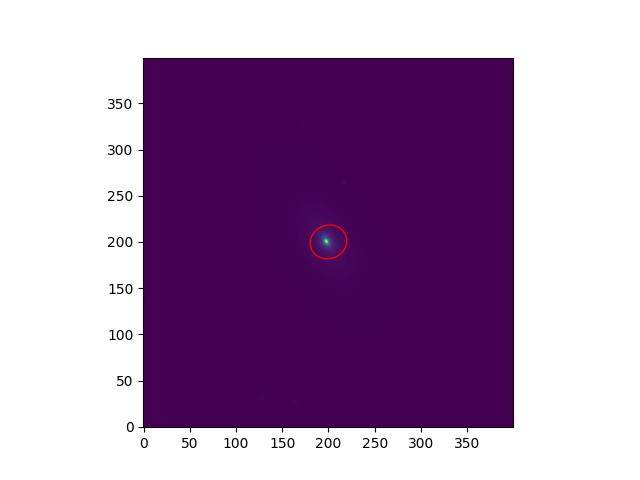
\includegraphics[scale=0.7]{imagens/initial0ngc3522}
	\caption{Elipse inicial}
\end{figure}

\begin{figure}[H]
	\centering
	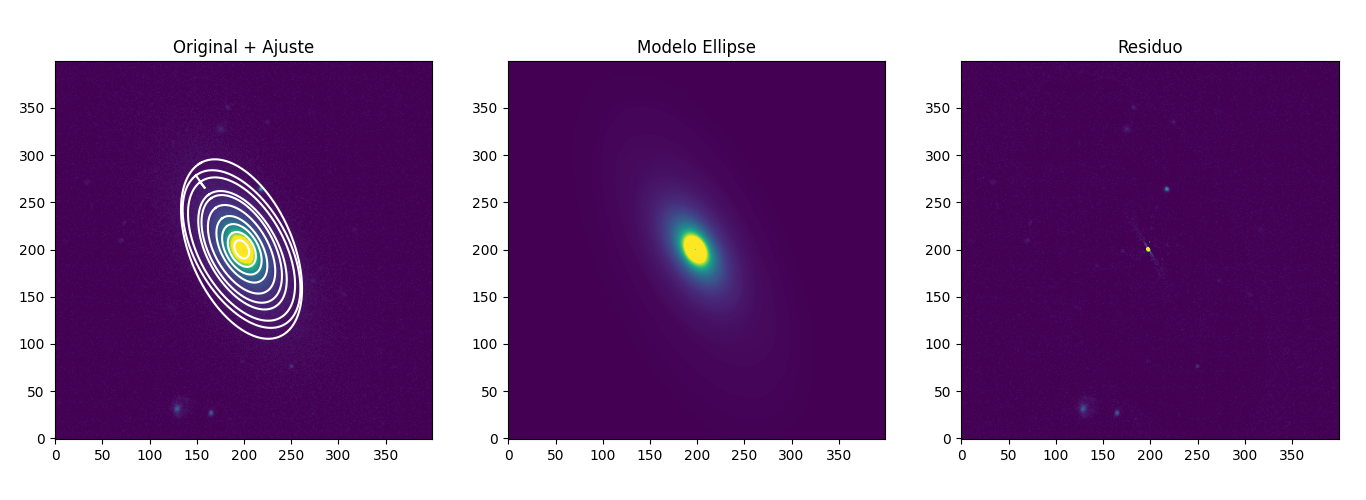
\includegraphics[scale=0.5]{imagens/isofotas0ngc3522}
	\caption{Isofotas de \textit{NGC 3522}}
\end{figure}

\begin{figure}[H]
	\centering
	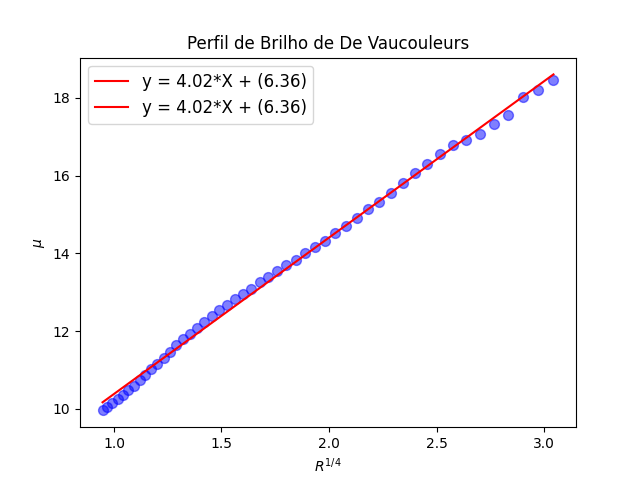
\includegraphics[scale=0.8]{imagens/linear0fit0ngc3522}
	\caption{Ajuste linear do perfil de brilho de \textit{NGC 3522}}
\end{figure}

\newpage
\subsection{Ajuste de \textit{NGC 5628}}

\begin{figure}[H]
	\centering
	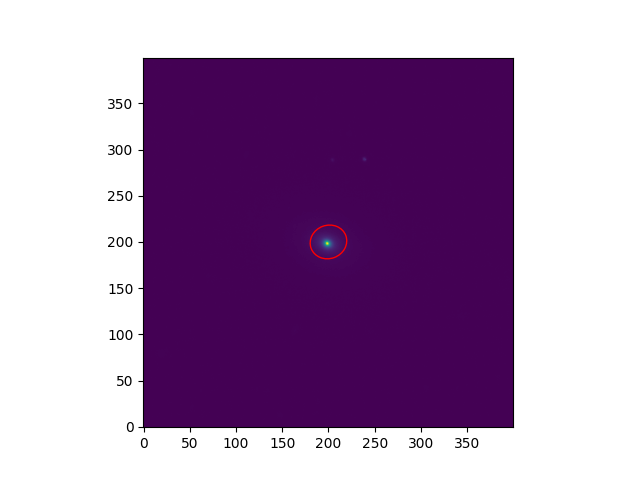
\includegraphics[scale=0.7]{imagens/initial0ngc5628}
	\caption{Elipse inicial}
\end{figure}

\begin{figure}[H]
	\centering
	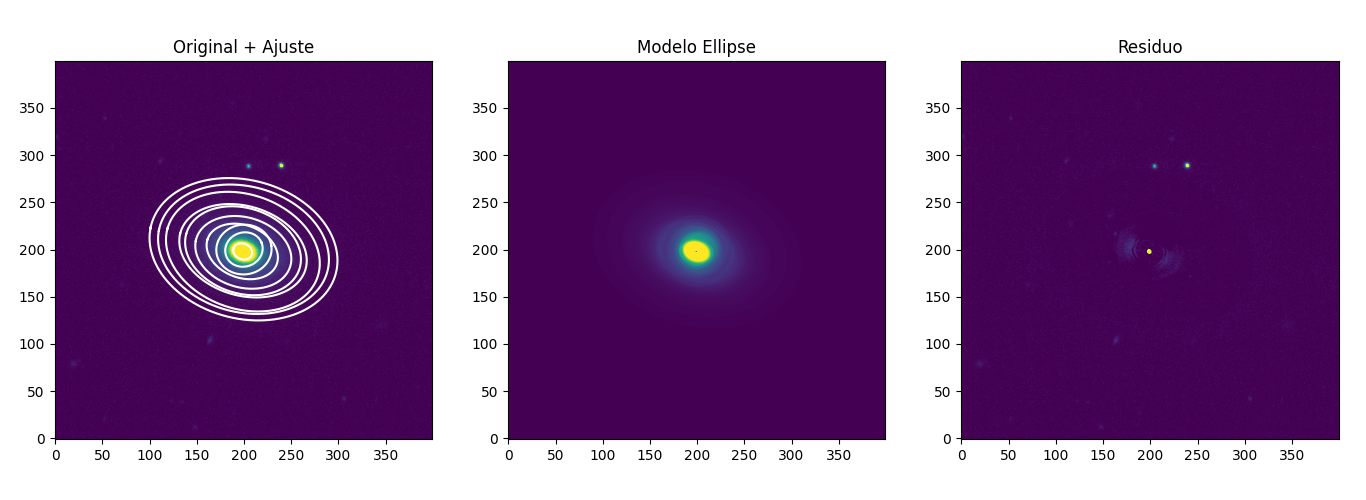
\includegraphics[scale=0.5]{imagens/isofotas0ngc5628}
	\caption{Isofotas de \textit{NGC 5628}}
\end{figure}

\begin{figure}[H]
	\centering
	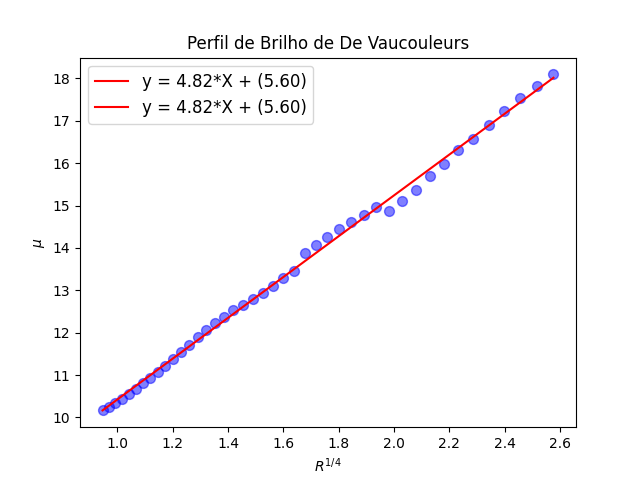
\includegraphics[scale=0.8]{imagens/linear0fit0ngc5628}
	\caption{Ajuste linear do perfil de brilho de \textit{NGC 5628}}
\end{figure}

\newpage
\subsection{Erros dos ajustes}

% Apresentação dos erros dos ajustes e detalhes estatísticos

\subsubsection{Erros do ajuste de \textit{NGC 3522}}

\begin{figure}[H]
	\centering
	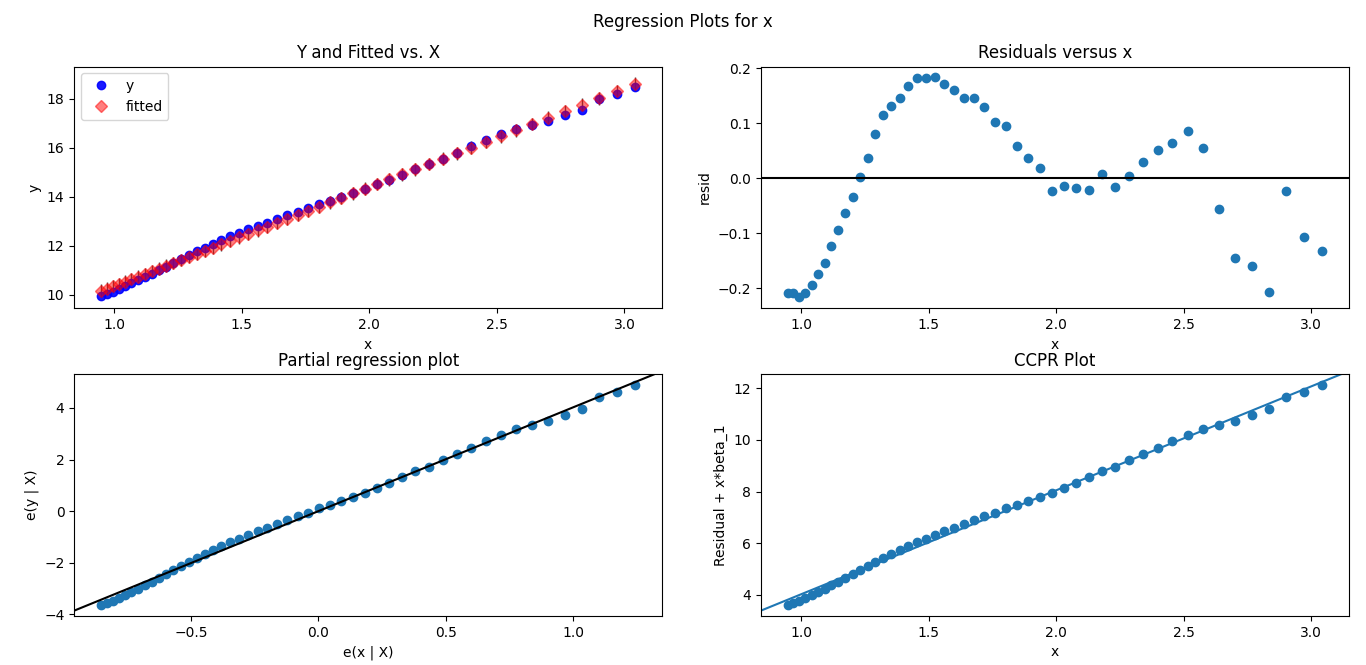
\includegraphics[scale=0.5]{imagens/regression0ngc3522}
	\caption{Regressão}
\end{figure}

\begin{figure}[H]
	\centering
	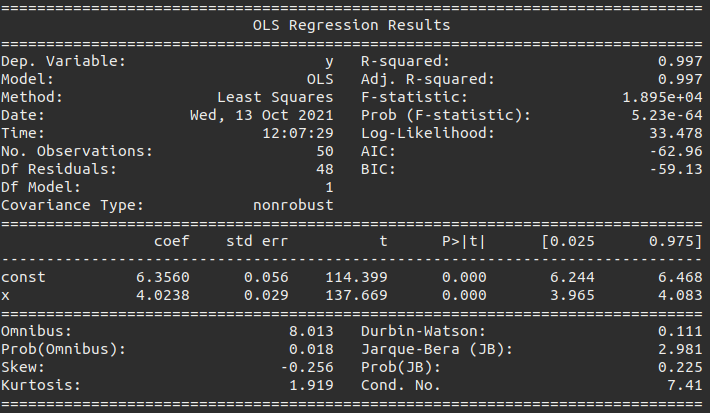
\includegraphics[scale=0.8]{imagens/data0ngc3522}
	\caption{Dados da Regressão Linear}
\end{figure}

\newpage
\subsubsection{Erros do ajuste de \textit{NGC 5628}}

\begin{figure}[H]
	\centering
	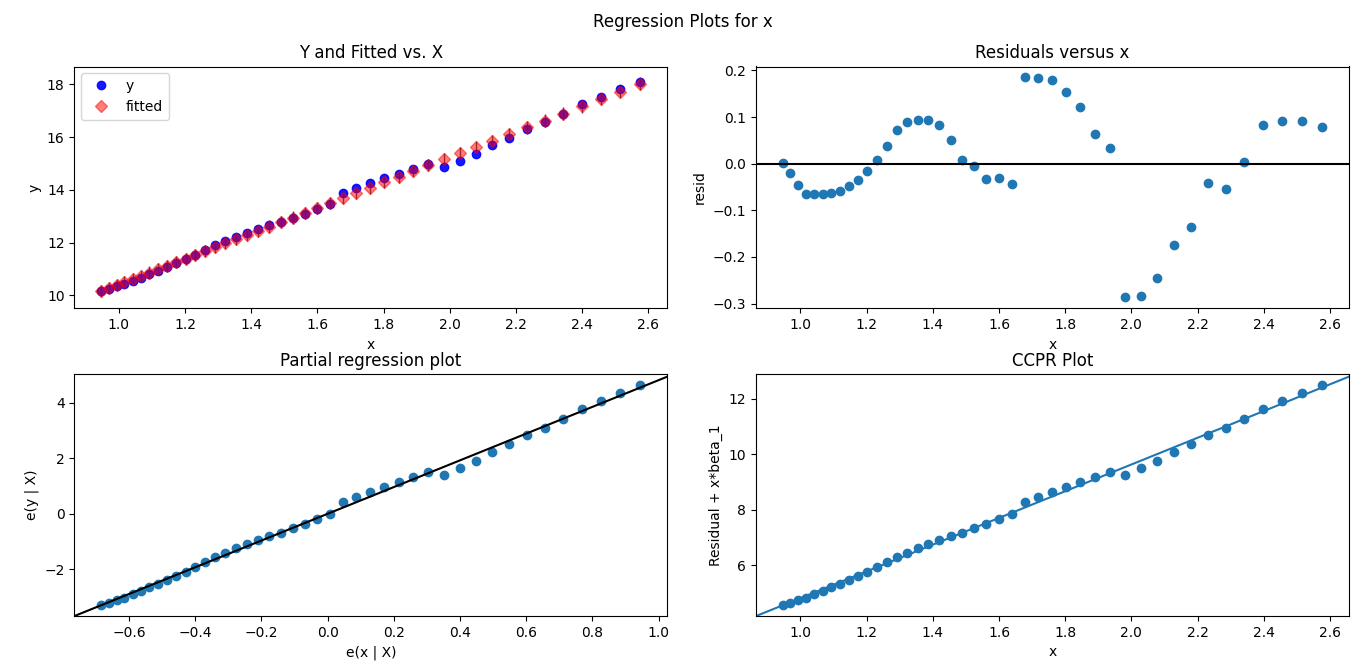
\includegraphics[scale=0.5]{imagens/regression0ngc5628}
	\caption{Regressão}
\end{figure}

\begin{figure}[H]
	\centering
	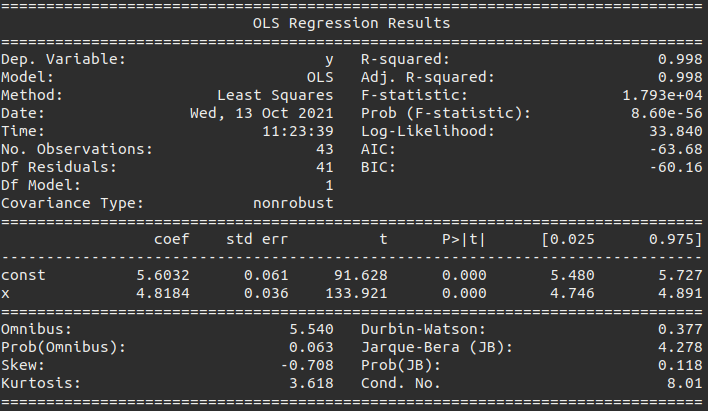
\includegraphics[scale=0.8]{imagens/data0ngc5628}
	\caption{Dados da Regressão Linear}
\end{figure}

\newpage
\noindent Com os coeficientes do ajuste foi possível calcular: \\

\begin{itemize}
	\item Brilho superficial interno: $\mu_{0} = a$;
	\item Intensidade isofotal interna: $I_{0}$;
	\item Intensidade isofotal no raio efetivo: $I_{eff}$;
	\item $\alpha$;
	\item Raio efetivo: $R_{eff}$;
	\item Luminosidade: $L$;
	\item Raio físico real: $r$.
\end{itemize}

\begin{table}[H]
	\centering
	\begin{tabular}{|c|c|c|}
	\hline 
	\textbf{Galáxia} & \textit{NGC 3522}  & \textit{NGC 5628} \\ 
	\hline 
	$\mu_{0}$ & $6.3559$ & $5.6031$ \\ 
	\hline 
	$I_{0}$ & $0.002868$ & $0.005737$ \\ 
	\hline 
	$I_{eff}$ & $1.3415 \cdot 10^{-6}$ & $2.6836 \cdot 10^{-6}$ \\ 
	\hline 
	$\alpha$ & $0.005300$ & $0.002578$ \\ 
	\hline 
	$R_{eff}$ & $18.3360$ & $8.9175$ \\ 
	\hline 
	$L ~ [L_{\odot}]$ & $0.01020$ & $0.00483$ \\ 
	\hline 
	$r ~ [kpc]$ & $2.0126$ & $3.7768$ \\ 
	\hline 
	\end{tabular} 
\end{table}

\subsection{Comparação com os dados da literatura}

\noindent Os valores de raio físico concordam razoavelmente com a database \textit{NASA/IPAC Extragalactic Database} (NED).\footnote{\url{https://ned.ipac.caltech.edu/}} Já os valores de luminosidade divergem muito.\\

\begin{figure}[H]
	\centering
	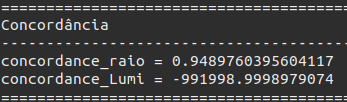
\includegraphics[scale=1]{imagens/concordanciangc3522}
	\caption{Concordância nos resultados de \textit{NGC 3522}}
\end{figure}

\begin{figure}[H]
	\centering
	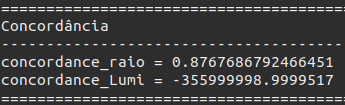
\includegraphics[scale=1]{imagens/concordanciangc5628}
	\caption{Concordância nos resultados de \textit{NGC 5628}}
\end{figure}

\section{Considerações Finais}

\noindent Os valores de luminosidade divergem muito dos encontrados na database \textit{NASA/IPAC Extragalactic Database} (NED).\footnote{\url{https://ned.ipac.caltech.edu/}} A explicação para isso se deve à provavelmente algum tipo de conversão necessária entre a luminosidade encontrada e a luminosidade bolométrica na banda específica do \textit{SLOAN}. \\

\noindent Apesar de não ter entendido a divergência dos resultados de luminosidade, este trabalho me fez aprender coisas muito interessantes: Foi meu primeiro contato, coletando dados do VizieR, meu primeiro contato com rotinas do IRAF e o poder da biblioteca astropy em vincular rotinas do IRAF com o python. Foi muito interessante entender como o python coleta a informação de intensidade isofotal e transforma em números associados a parâmetros da elipse. Outro ponto importante foi o contato com o survey do SLOAN e o ds9.\\

\noindent Foi particularmente curioso testar ajustes de isofotas em distintas imagens de galáxias: algumas com sinais de interação ou núcleo ativo foram "facilmente resolvidas". É impressionante como o ajuste isofotal separa as estruturas e revela a parte mais interna das galáxias com disco, ou ainda, revela estrututas mais externas, remanescentes de colisão de galáxias. Em meio à busca de imagens, o campo de \textit{NGC 7317}, em especial, chamou muito a atenção, porém, nada viável à aplicação do ajuste do perfil de brilho de De Vaucouleurs. \\

\section{Referências}

\begin{itemize}
	\item [1] \url{https://vizier.cds.unistra.fr/viz-bin/VizieR?-source=VII/155}
	\item [2] \url{http://skyserver.sdss.org/dr8/en/tools/explore/}
	\item [3] \url{https://ds9.si.edu/}
	\item [4] \url{http://simbad.u-strasbg.fr/simbad/}
	\item [5] \url{https://ned.ipac.caltech.edu/}
	\item [6] Peter Scheneider
	\item [7] Notas de aula: Prof. Oscar Cavichia, UNIFEI.
\end{itemize}

\newpage
\section{Apêndice}

\subsection{Código que ajusta as isofotas às imagens}

\small{
\begin{lstlisting}[language=Python]
	
#!/usr/bin/python
# -*- coding: utf-8 -*-

__author__ = 'Oscar Cavichia'


import sys
import numpy as np
import matplotlib.pyplot as plt

import astropy

from astropy.modeling.models import Gaussian2D
from astropy.io import fits
from astropy.nddata import Cutout2D
from astropy.wcs import WCS

#!pip3 install photutils

import photutils

from photutils.datasets import make_noise_image
from photutils.isophote import EllipseGeometry
from photutils.aperture import EllipticalAperture
from photutils.isophote import Ellipse
from photutils.isophote import build_ellipse_model

def main(argv=None):
    
#Substituir a imagem abaixo pela sua
  
   imageFile = "NGC3522_SDSSr.fits.bz2"
	
# https://vizier.u-strasbg.fr/viz-bin/VizieR-4
# http://skyserver.sdss.org/dr8/en/tools/explore/obj.asp?ra=166.6708&dec=20.0856
# RA: 166.6708 deg / DEC: 20.0856 deg
# http://simbad.u-strasbg.fr/simbad/sim-basic?Ident=NGC+3522&submit=SIMBAD+search
# https://ned.ipac.caltech.edu/byname?objname=NGC+3522&hconst=67.8&omegam=0.308&
omegav=0.692&wmap=4&corr_z=1
    
    hdul = fits.open(imageFile)
    #hdul.info()
    
    hdu=fits.open(imageFile)[0]
    
    image_data=hdu.data
    
    wcs = WCS(hdu.header)
    
#Verificar no ds9 as coordenadas x0 e y0 da galaxia e mudar os valores:
    
    position = (1709.39, 630.338)
    	size = (400, 400)
    
    	cutout = Cutout2D(image_data, position=position, size=size, wcs=wcs)
    	image_data_cut = cutout.data
    
    	plt.imshow(image_data_cut, origin='lower', cmap='viridis', vmin=0,vmax=1)
    
#Caso mude os valores de size, substituir x0 e y0 abaixo pela metade dos valores

geometry = EllipseGeometry(x0=200, y0=200, sma=20, eps=0.1, pa=20.*np.pi/180.)

aper = EllipticalAperture((geometry.x0, geometry.y0), geometry.sma, 

geometry.sma*

(1 - geometry.eps), geometry.pa)
    
plt.imshow(image_data_cut, origin='lower')
    
    aper.plot(color='red')

#Criamos uma instancia da classe Ellipse para fazer o ajuste de isofotas elipticas
    
	ellipse = Ellipse(image_data_cut, geometry)
    
#Fazemos o ajuste da elipse com o metodo fit_image. Nao ajustamos em menos de 2 pixels.
    
    	isolist = ellipse.fit_image(minsma=2)
    
#O resultado eh o objeto isolist que contem os atributos:

#https://photutils.readthedocs.io/en/stable/api/photutils.isophote.IsophoteList.html
#photutils.isophote.IsophoteList
    
#Vamos imprimir os semieixos das isofotas
    
    	print("sma = {0} \n intens = {1}".format(isolist.sma,isolist.intens))

#Os nomes de cada coluna sao:
    
    #print(isolist.get_names())

#Podemos imprimir uma tabela ordenada por sma:
    
    #print(isolist.to_table())
    
#Vamos salvar a tabela em uma arquivo txt
    
    	from tabulate import tabulate
    
    	with open('dados_ajuste.txt', 'w') as f:
    		f.write(tabulate(isolist.to_table(["sma","intens"])))
    
#Construir uma imagem do modelo
    
    	model_image = build_ellipse_model(image_data_cut.shape, isolist)
    
    	residual = image_data_cut - model_image
    
    	fig, (ax1, ax2, ax3) = plt.subplots(figsize=(14, 5), nrows=1, ncols=3)
    
    	fig.subplots_adjust(left=0.04, right=0.98, bottom=0.02, top=0.98)
    
    ax1.imshow(image_data_cut, origin='lower',cmap='viridis',vmin=0,vmax=2)
    
    ax1.set_title('Original + Ajuste')
    
    	smas = np.linspace(10, 100, 10)
    
    	for sma in smas:
    		iso = isolist.get_closest(sma)
        
        x, y, = iso.sampled_coordinates()
        
        ax1.plot(x, y, color='white')
    
    ax2.imshow(model_image, origin='lower',cmap='viridis',vmin=0,vmax=2)
    ax2.set_title('Modelo Ellipse')

	ax3.imshow(residual, origin='lower',cmap='viridis',vmin=0,vmax=2)
	ax3.set_title('Residuo')
    
    	plt.show()
    
    	return 0
    	
if __name__ == "__main__":
    sys.exit(main())
    
\end{lstlisting}
}

\newpage
\subsection{Código do ajuste linear e resultados}

\small{
\begin{lstlisting}[language=Python]

#!/usr/bin/python
# -*- coding: utf-8 -*-

__author__ = 'Rafael Passos Domingues'


import sys
import numpy as np
import matplotlib.pyplot as plt

import scipy as sp
import pandas as pd
import statsmodels.api as sm

def concordance(database,measured):
    
    c = 1 - (database - measured)/100
    
    return c

def linearfit(X,Y):

    # Linear Fit

    # create data
    df = pd.DataFrame({'x': X, 'y': Y})

    # fit simple linear regression model
    y = df['y']
    x = df['x']
    x = sm.add_constant(x)
    model = sm.OLS(y, x).fit()

    # view model summary
    print('=' * 78)
    print(model.summary())

    # produce residual plots
    fig = plt.figure(figsize=(12, 8))
    fig = sm.graphics.plot_regress_exog(model, 'x', fig=fig)

    plt.show()

    # regression part
    slope, intercept = model.params[1], model.params[0]

    line = slope * x + intercept
    plt.plot(x, line, 'r', label='y = {:.2f}*X + ({:.2f})'.format(slope, intercept))
    plt.legend(fontsize=12)

    # create scatterplot
    plt.scatter(df.x, df.y, color='blue', s=50, alpha=.5)
    plt.title('Perfil de Brilho de De Vaucouleurs')
    plt.xlabel('$R^{1/4}$')
    plt.ylabel('$\mu$')

    plt.show()

    return slope,intercept

def main(argv=None):
    
    # Dados
    
    dados = pd.DataFrame(
    [[float(token) for token in line.split()]  
        for line in open("dados_ajuste.txt") if line.strip()],
     columns = ["sma", "intens"]
     )
    
    sma = np.array(dados['sma']) # X
    intens = np.array(dados['intens']) # Y
    
    # Conversoes -- [px -> arcsec] & [nmgy -> Jy]
    sma = sma * (0.39597) # [arcsec]
    intens = intens * (3.631 * 10**(-6)) # [Jy]
    
    # Semieixos maiores ajustados, elevados a (1/4)
    R14 = sma**(.25) # R**(1/4) # [arcsec**(1/4)]
    
    # Brilho superficial
    mu = -2.5 * np.log10(intens)
    
    # --- --- ---
    
    # Coeficientes do ajuste
    slope, intercept = linearfit(R14,mu)

    print('\n')
    print('=' * 78)
    print('Coeficientes')
    print('-' * 78)
    print('slope = {0}'.format(slope))
    print('intercept = {0}'.format(intercept))
    print('=' * 78)
    print('\n')
    
    # --- --- ---
    
    # Resultados
    
    mu_0 = intercept
    I_0 = 10**(-(2/5) * intercept)
    
    # Magnitude Bolometrica do Sol
    # Ref: https://www.astro.princeton.edu/~gk/A403/constants.pdf
    Mbol_sun = 4.74
    
    I0 = 10**((Mbol_sun + 21.572 - mu_0)/(2.5)) # [L_sun]
    I_e = 10**(-3.33) * I_0
    
    alpha = ((2.5)/(slope * np.log(10)))**(4)
    R_eff = 3459 * alpha
    
    distance = 22.64 * 10**(3) # [kpc] # 22.64 +/- 1.62 [Mpc] (CMB)
    theta = R_eff * (4.84814 * 10**(-6)) # [rad]
    r = distance * np.sin(theta) # [kpc]
    
    R_opt = 2.5 * R_eff # Raio optico
    
    # Luminosidade
    
    n = 4 # galaxia eliptica
    j = 2*n
    fat = 1
    i = 2
    while i <= j:
        fat = fat*i
        i = i + 1

    L = fat * np.pi * I_0 * alpha**(2)
    
    # Area dos pixels
    A = (0.39597)**(2)
    
    # Brilho superficial efetivo
    mu_eff = 22.5 - 2.5 * np.log10(intens) + 2.5 * np.log10(A) # [mag/arcsec**2]
    
    print('=' * 78)
    print('Resultados')
    print('-' * 78)
    
    print('mu_0 = {0}'.format(mu_0))
    print('I_0 = {0}'.format(I_0))
    print('I0 = {0} [L_sun]'.format(I0))
    print('I_e = {0}'.format(I_e))
    
    print('alpha = {0}'.format(alpha))
    print('R_eff = {0} [kpc]'.format(R_eff))
    print('r = {0} [kpc]'.format(r))
    print('R_opt = {0} [kpc]'.format(R_opt))
    
    print('L = {0} [L_sun]'.format(L))
    
    print('mu_eff = {0} [mag/arcsec**2]'.format(mu_eff))
    
    print('=' * 78)
    print('\n')
    
    # Concordance
    
    concordance_r = concordance(14.23/2,r)
    concordance_L = concordance(9.92E7,L)
    
    print('=' * 78)
    print('Concordancia')
    print('-' * 78)
    
    print('concordance_raio = {0}'.format(concordance_r))
    print('concordance_Lumi = {0}'.format(concordance_L))
    
    print('=' * 78)
    print('\n')
    
    return 0

if __name__ == "__main__":
    sys.exit(main())

\end{lstlisting}
}

\end{document}
